\documentclass[a4paper, 11pt, oneside]{book}

\usepackage{amsthm} %per teorema
\usepackage{tikz-cd}
\usepackage{drawstack}
\theoremstyle{plain}
\usetikzlibrary{calc}
\usepackage[utf8]{inputenc}
\usepackage[T1]{fontenc}
\usepackage[magyar]{babel}
\usetikzlibrary{positioning, shapes}
\usepackage{graphicx}
\usepackage{graphicx,changepage}
\usepackage{graphicx}
\usepackage{grffile}



\newlength\Textwd
\setlength\Textwd{3cm}
\newcommand\Textbox[2]{%
  \parbox[c][#1][c]{\Textwd}{\centering#2}}



\begin{document}



\chapter*{2\\IL LIVELLO APPLICATIVO} 

\section*{Introduzione}

In questo capitolo verranno analizzati alcuni protocolli facenti parte di entrambi i modelli standard di rete informatica: il modello \textit{OSI} ed il modello\textit{ TCP/IP}. \\
Benché lo standard internazionale per la comunicazione sia rappresentato dal modello OSI, questo è utilizzato più come un modello astratto di riferimento. Nella pratica comune lo standard è il modello TCP/IP, caratterizzato da un numero inferiore di livelli di rete e da una conseguente elevata praticità. 

\begin{center}
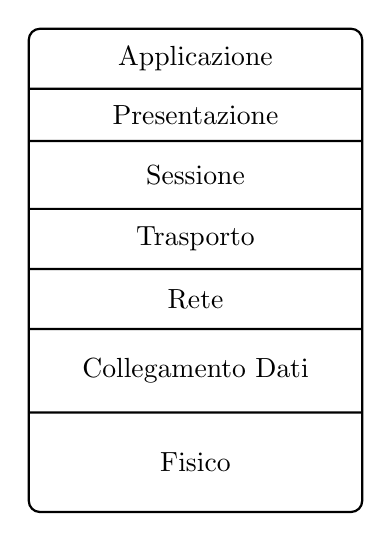
\begin{tikzpicture}[auto,
rect/.style={
  rectangle split, rectangle split parts=7,
  draw, thick, rounded corners,
  text width=4cm,
  text centered,
  rectangle split part fill={white}
}]
\node (stack) [rect] {
\nodepart {one} \Textbox{0.5cm}{Applicazione}
\nodepart {two} \Textbox{0.4cm}{Presentazione}
\nodepart{three} \Textbox{0.6cm}{Sessione}
\nodepart{four}\Textbox{0.5cm}{Trasporto}
\nodepart{five} \Textbox{0.5cm}{Rete}
\nodepart{six} \Textbox{0.8cm}{Collegamento Dati}
\nodepart{seven} \Textbox{1cm}{Fisico}
};
\end{tikzpicture} 
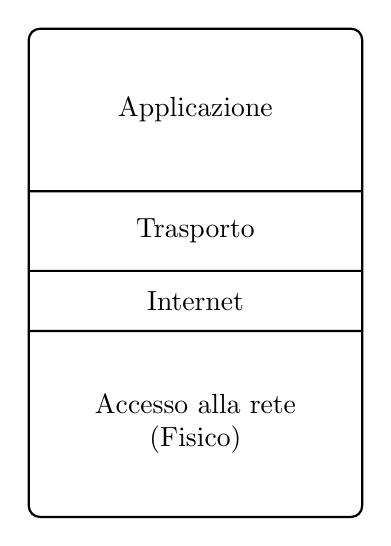
\begin{tikzpicture}[auto,
rect/.style={
  rectangle split, rectangle split parts=4,
  draw, thick, rounded corners,
  text width=4cm,
  text centered,
  rectangle split part fill={white}
}]
\node (stack) [rect] {
\nodepart {one} \Textbox{1.80cm}{Applicazione}
\nodepart {two} \Textbox{0.75cm}{Trasporto}
\nodepart{three} \Textbox{0.5cm}{Internet}
\nodepart{four}\Textbox{2.10cm}{Accesso alla rete (Fisico)}
};
\end{tikzpicture}
\end{center}
\begin{center}
 Figura 2.1. \textit{Richiamo alla struttura dei modelli ISO/OSI (sinistra) e TCP/IP (destra).}
\end{center}


I livelli OSI riguardati da questa modifica sono i livelli che andremo ad analizzare in questo capitolo, definendoli ed approfondendone i principali servizi. Il \textit{livello applicativo} (o applicazione) è il settimo e più esterno livello nel modello OSI ed il quarto e ultimo livello nel TCP/IP. Il parallelismo di tale strato nei due standard sarà motivo di studio nelle sezioni successive.\\
Prima di andare ad approfondire i servizi offerti dai vari livelli dei due standard, si tratterà di come si sono sviluppate le \textit{applicazioni web}, a partire dalla nascita di internet fino ad arrivare ad oggi, in modo da avere un quadro generale dello sviluppo delle tecnologie che hanno permesso e permettono tutt'ora, l'evoluzione della rete.

\section*{2.1 Funzionalità}
Il livello applicazione è un livello astratto che ha la funzione di specificare all'interno di una rete le interfacce ed i protocolli di comunicazione utilizzati e più in generale di fornire servizi alle applicazione degli utenti della rete, al fine di garantire una corretta trasmissione.\\\\
Quando due programmi devono comunicare tra loro è necessario prima di tutto che esista una connessione logica tra le due entità logiche (mittente e ricevente). Tramite essa si può andare a gestire i quattro livelli dello \textit{stack TCP/IP} per mezzo di un insieme di istruzioni (o funzioni) denominate \textit{API} (\textit{Application Program Interface}) che ci permettono di aprire e chiudere connessioni ed inviare e ricevere dati. \\Durante una trasmissione ogni strato dello stack aggiunge un header al pacchetto dati che identifica il messaggio da trasmettere. Questa operazione è chiamata \textbf{incapsulamento}. Per mezzo di essa è possibile identificare il dato effettivo e l'header aggiunto dallo strato attuale come un unico pacchetto dati che verrà successivamente passato allo strato sottostante. Il pacchetto risultante dal passaggio dell'intero stack verrà poi trasmesso e ricevuto. Il computer o l'applicazione ricevente dovrà poi effettuare l'operazione inversa, estraendo ad ogni livello l'header necessario a dirigere l'operazione di ricezione.
\\\\Il primo e più esterno strato dello stack, come anticipato, è il livello applicativo, il quale ha lo scopo di \textit{standardizzare la comunicazione}. Nel TCP/IP infatti, il livello applicativo contiene i protocolli e le interfacce di comunicazione usati nelle trasmissioni processo a processo per completare le varie richieste dei programmi, svolte attraverso il protocollo internet (IP), all'interno di una rete. Tra i protocolli più comunemente usati troviamo HyperText Transfer Protocol (HTTP), File Transfer Protocol (FTP), Domain Name System (DNS) e Simple Mail Transfer Protocol (SMTP).\\
Un esempio di concreto utilizzo dei protocolli si ha ogni volta che richiediamo al nostro browser di accedere ad internet o di caricare o scaricare qualcosa da esso. Il livello applicativo per completare la richiesta, chiamerà nel primo caso il protocollo HTTP mentre nel secondo il protocollo FTP.\\
Per far arrivare all'utente i dati richiesti secondo lo standard TCP/IP, il livello applicazione deve passare i dati al livello trasporto attraverso degli indirizzi ( o interfacce ) logici chiamati \textit{porte}. Sarà poi il\textit{ livello trasporto} ad occuparsi della ricezione finale da parte dell'utente.\\
L'utilizzo delle porte rende molto più semplice al livello trasporto, capire che tipo di dato gli sta venendo passato. Se ad esempio venisse inviato un dato sulla porta 25, significherebbe che il dato riguarda una richiesta e-mai. Se invece fosse stato mandato sulla porta 21 o 22, sarebbe stato un dato FTP.\\\\ 
Il livello applicazione nel TCP/IP non specifica nessun tipo di regola o formato di dati accettabili, che le applicazioni devono invece tenere di conto durante le trasmissioni. Per questo motivo nella specifica iniziale dello standard è fortemente raccomandato di seguire il \textbf{robustness principle} (principio di robustezza). \\

\newtheorem*{theorem*}{Principio di robustezza}
\begin{theorem*}
(o legge di Postel): “be conservative in what you do, be liberal in what you accept from others”.
 \end{theorem*} 
 In altre parole, quando viene inviato un messaggio 			ad un altro computer o ad un'altra applicazione, questo deve essere perfettamente conforme alla specifica richiesta. In caso invece di messaggi in entrata non conformi, questi devono essere accettati fintanto che il loro significato è chiaro.\\\\
Nel modello OSI il livello applicativo è costituito, come nel TCP/IP, da un insieme di protocolli ed interfacce di comunicazione tra i quali HTTP, FTP, DNS e SMTP. Una sostanziale differenza però la si trova nella struttura stessa del modello. Il livello applicativo del TCP/IP comprende sia il livello applicativo che i livelli presentazione e sessione del modello OSI. Questa maggiore modularità degli strati dello standard OSI è dovuta ad una più elevata distribuzione delle funzioni tra essi. Il livello applicazione del modello OSI, lavora infatti direttamente col software applicativo e si occupa "solo" di verificare la effettiva disponibilità di un partner per la comunicazione e delle risorse necessarie alla trasmissione. Una volta appurata la presenza di un partner e la disponibilità di risorse, il pacchetto dati composto dal dato da scambiare e dall'header aggiunto dal livello applicazione viene passato al sottostante livello presentazione.

\section*{2.2 Livelli Presentazione e Sessione}
\textbf{Il livello presentazione} è il sesto livello del modello ISO/OSI ed è il primo livello ad occuparsi del significato delle informazioni trasmesse. Ha la funzione di assicurare la compatibilità dei dati durante una comunicazione tra entità che utilizzano codifiche diverse. Questo avviene tramite una traduzione del dato in una forma accettabile (quindi comprensibile) dal livello applicazione e dai livelli sottostanti del ricevente. Nello specifico: una volta iniziata la trasmissione, cambia il formato dei dati da quello del dispositivo mittente (\textit{sintassi locale}, a quello del dispositivo ricevente (\textit{sintassi di trasferimento}\\Questo strato offre inoltre importanti servizi quali la formattazione, la codifica, la criptazione e la compressione di dati. Se ad esempio si volesse convertire un file di testo scritto in EBCDIC (Extended Binary Coded Decimal Interchange Code) in un file scritto in  ASCII (American Standard Code for Information Interchange), tale conversione avverrebbe a questo livello. Un altro esempio si ha quando si invia un file di testo dal contenuto sensibile (come una password), ed è dunque necessario che il messaggio venga criptato. Tale operazione avviene proprio al livello presentazione. \\Una volta finita l'elaborazione del pacchetto dati questo viene passato allo strato inferiore, il livello sessione.\\\\
\textbf{Il livello sessione} è il quinto livello del modello OSI e fornisce i meccanismi per stabilire, gestire ed infine concludere una comunicazione (o sessione) tra una applicazione locale ed una remota, svolgendo inoltre un'operazione di verifica per assicurarsi della corretta ricezione del pacchetto dati. È solo a questo punto dello stack infatti, dopo che il livello applicativo e presentazione hanno fornito i protocolli necessari ed adattato il pacchetto dati alla comunicazione che avviene la connessione, permettendo agli strati inferiori di attuare l'effettivo invio del pacchetto dati. In base alla durata della sessione è possibile classificare le diverse tipologie di comunicazione. Una trasmissione si definisce \textbf{simplex}, quando la sessione dura al massimo il tempo necessario ad inviare un solo messaggio in una direzione. Un'altra modalità è la \textbf{half-duplex}, e si ha quando la trasmissione è sufficientemente lunga per una comunicazione bidirezionale ma capace di gestire un solo messaggio alla volta. L'ultima e più recente modalità è la \textbf{full-duplex}, la quale permette una comunicazione bidirezionale e simultanea. \\ Essendo comunque le comunicazioni generalmente brevi, il quinto livello fu dotato della capacità di instaurare un \textit{ponte di comunicazione} semi permanente tra due entità per ottimizzare la qualità delle trasmissioni a lungo termine e per meglio gestire le comunicazioni simultanee di applicazioni web.\\ Nel modello TCP/IP tuttavia questo livello non è presente e le modalità di instaurazione di una comunicazione tra due entità possono risultare più complesse. Il livello sessione è stato inglobato in parte nel livello trasporto ed in parte nel livello applicativo, caratterizzando quest'ultimo in fase di apertura di una trasmissione, con una\textit{ struttura stratificata}. Quando infatti si va ad invocare una pagina web tramite un browser, nel TCP/IP i protocolli necessari alla visualizzazione di essa vengono impilati dalla cima dello stack TCP/IP seguendo un ordine crescente di potenza del servizio offerto. Se ad esempio dovessimo caricare una pagina web per guardare un programma in streaming, il livello applicativo impilerebbe tutti i protocolli necessari alla visualizzazione di essa partendo dal più semplice HTTP, fino ad arrivare al RTP(Real-time Trasmission Protocol) (Figura 2.2).
\begin{center}
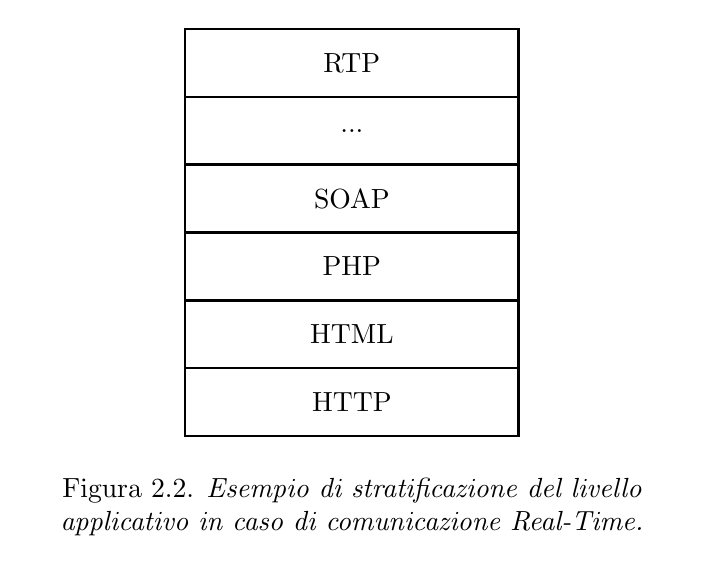
\begin{tikzpicture}[auto,
rect/.style={
  rectangle split, rectangle split parts=6,
  draw, thick,
  text width=4cm,
  text centered,
  rectangle split part fill={white}
}]

\node (stack) [rect] {
\nodepart {one} \Textbox{0.6cm}{RTP}
\nodepart {two} \Textbox{0.6cm}{...}
\nodepart{three} \Textbox{0.6cm}{SOAP}
\nodepart{four}\Textbox{0.6cm}{PHP}
\nodepart{five} \Textbox{0.6cm}{HTML}
\nodepart{six} \Textbox{0.6cm}{HTTP}

};
\node [below=3cm, align=flush center,text width=8cm] at (stack)
        {
            Figura 2.2. \textit{Esempio di stratificazione del livello applicativo in caso di comunicazione Real-Time.}
        };
\end{tikzpicture} 
\end{center}
A livello sessione vengono gestite anche le funzioni di autenticazione e autorizzazione e viene fornito il servizio di \textit{session restoration} (checkpointing and recovery). Quest'ultimo servizio proverà, in caso di perdita di connessione, a ripristinarla riavviando se necessario la comunicazione.\\ Un esempio dei servizi offerti dal livello sessione si ha durante una video chiamata, durante la quale è essenziale che il video e l'audio siano sincronizzati per evitare \textit{problemi di lip synch} (problemi di sincronizzazione del movimento delle labbra con l'audio). Se il quinto strato è ben progettato, la persona sullo schermo corrisponderà sempre all'audio in uscita, ed in caso di perdita di connessione, il meccanismo di session restoration, proverà a ristabilirla. \\Date le sue caratteristiche, il livello sessione veniva tipicamente implementato negli ambienti applicativi che facevano uso delle RPCs (chiamate a procedura remote), ma soprattutto nei Web browsers. In questi ultimi sfruttava comunemente protocolli come lo ZIP (Zone Information Protocol) ed il SCP(Session Control Protocol).
\section*{2.3 Evoluzioni delle applicazioni Internet e Web}
Dalla nascita di \textit{ARPANET} negli anni '60 si sviluppò nel mondo un nuovo modo di comunicare: la rete internet. Sebbene inizialmente i fini fossero puramente militari, con la fine della Guerra Fredda l'esercito si disinteressò dello strumento, lasciandolo nel pieno controllo delle università dove divenne utile per scambiare conoscenze scientifiche e più in generale per comunicare. Negli stessi anni \textit{Tim Berners-Lee} creò un'architettura che semplificò drasticamente l'utilizzo della rete ormai rinominata Internet: il \textbf{World Wide Web.}\\Nel 1991 lo stesso Tim Berners-Lee, creò il primo sito web, avviando una rivoluzione che oggi chiamiamo \textbf{Web 1.0}.\\\\
Il Web 1.0 era l'internet dei contenuti, caratterizzato da siti web semplici e statici dai quali era possibile solo accedere a risorse senza poterle modificare o aggiungere. Le pagine web erano scritte da una ristretta cerchia di persone ed erano gremite di collegamenti ipertestuali (link) ad altre pagine, in modo da dare all'utente più libertà di movimento possibile all'interno della rete. È col Web 1.0 che nacque il concetto di \textit{applicazione internet} (web application), cioè un programma di tipo client-server che viene eseguito dal client tramite un \textit{web browser}. Nel Web 1.0 il client, rappresentato dal browser, per mezzo di uno o più web server accedeva a pagine web statiche le quali comunicando con dei semplici server, restituivano il contenuto desiderato.
\begin{center}
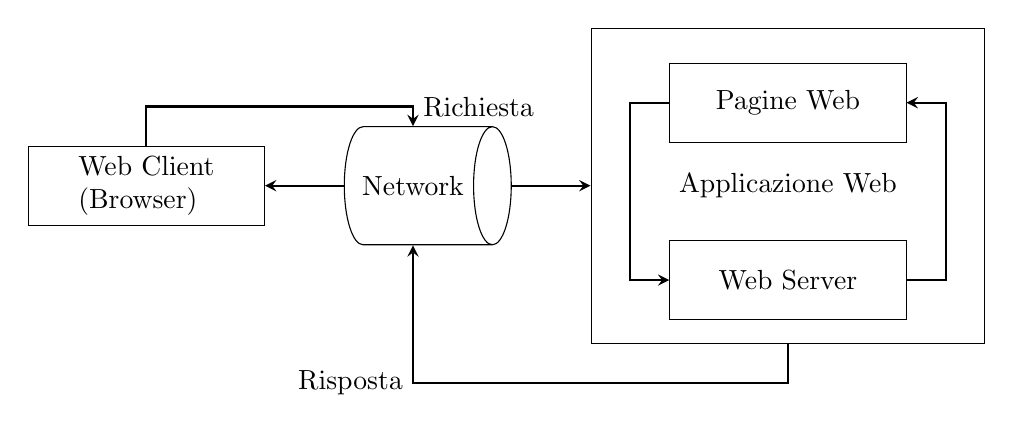
\begin{tikzpicture}[auto,
  node distance = 0.5cm and 1cm, text centered,
 entity/.style = {rectangle, draw,
                   minimum width=3cm, minimum height=1cm, align=left},
net/.style = {cylinder, draw,
                   minimum width=1.5cm, minimum height=1cm, align=left, draw=black}, wapp/.style = {rectangle, draw,
                   minimum width=5cm, minimum height=4cm},
   arrow/.style = {thick,-stealth}
                    ]
\node (client)  [entity] {Web Client\\(Browser)};
\node (network)  [net,right=of client]   {Network};
\node (server) [wapp, right=of network]  (main) {Applicazione Web};
\node(webS) [entity] at ([yshift=2.3em]main.south){Web Server};
\node(webP) [entity] at ([yshift=3em]main.center){Pagine Web};
% connections

\draw [arrow] (client.north) --+ (0,0.5) -| (network) node[midway,sloped,right, rotate=90] {Richiesta};;
\draw [arrow] (network) -- (client);
\draw [arrow] (network) -- (main);
\draw [arrow] (webS.east) -- + (0.5,0) |- (webP);
\draw [arrow] (webP.west) --+  (-0.5,0) |- (webS);
\draw [arrow] (main.south) --+  (0,-0.5) -| (network) node[midway,sloped,left,rotate=270] {Risposta};
\end{tikzpicture}

\begin{tikzpicture}
\node [align=center,text width=13cm]
        {
           \\Figura 2.3. \textit{Modello semplificato della struttura del Web 1.0}
        };
\end{tikzpicture}
\end{center}
I browser utilizzati per la navigazione erano molto semplici poiché l'unico linguaggio che dovevano interpretare era l'HTML. Nel Web 1.0 non era inoltre prevista alcun tipo di separazione tra i dati e la loro rappresentazione, era tutto semplicemente ammassato nelle pagine web, rendendo queste ultime molto fragili. Se ad esempio doveva essere cambiata anche solo una parola, si doveva andare a modificare l'intera pagina.  \\Le comunicazioni erano gestite solo dal protocollo HTTP, tutt'oggi ancora fondamentale. Questo ha la caratteristica di essere un protocollo\textit{ senza stato} (state-less protocol), che cioè tratta ogni richiesta da client a server in modo indipendente dalle altre causando di conseguenza la perdita di qualsiasi informazione scambiata tra browser e server al termine della trasmissione. Se ad esempio avessimo messo qualcosa nel carrello di un qualche sito di acquisti ed avessimo poi navigato su altri siti o chiuso e riaperto il collegamento, una volta tornati al nostro sito di acquisti avremmo trovato il carrello vuoto. Questo problema venne risolto sempre in quel periodo con l'invenzione dei \textbf{cookies}. Per mezzo di essi, ogni volta che l'utente effettuava una richiesta il browser, se necessario, inviava al server i cookies per notificarlo di connessioni precedenti.\\\\
Col progredire degli anni e l'aumentare del numero degli utenti, si rendeva sempre più necessaria la possibilità di interagire con i contenuti. Il mutamento iniziò grazie all'ausilio dei nuovi linguaggi di programmazione come \textit{PHP}, per mezzo dei quali iniziarono a crearsi i primi \textit{blog}, cioè siti web sui quali era possibile inserire dei commenti. Questo primo cambiamento comportò l'avvento delle prime \textit{community} e venne identificato come \textbf{Web 1.5}. \\Di lì a pochi anni la rete si espanse in modo esponenziale con l'introduzione dei \textit{Wiki} e dei \textit{Social Network}, ponendo l'interattività con l'utente in primo piano e facendo nascere così il\textbf{ Web 2.0}.\\\\
La rete da statica divenne quindi dinamica, apportando modifiche architetturali principalmente lato server, rendendolo decisamente più complesso. Non si avevano più semplici pagine web statiche che reperivano informazioni da server, ma pagine web dotate di un elevato numero di servizi e script costantemente in comunicazione con qualche \textit{database} (Fiugura 2.4). \\ Due dei servizi più innovativi furono gli \textit{RSS} ed i \textit{Podcast}. L'RSS (Really Simple Syndacation) è uno dei più popolari formati di distribuzione dei contenuti web basato su XML (eXtensible Markup Language) per mezzo del quale divenne possibile, tramite il meccanismo di feed-RSS, monitorare gli aggiornamenti di un sito senza visitarlo. La funzionalità dei Podcast è molto simile, ma anziché monitorare il cambiamento di testo ed immagini, tramite tale meccanismo si rese possibile monitorare l'inserimento di file audio e video.\\
\begin{center}
\resizebox{13cm}{!}{
\begin{tikzpicture}[auto,
  node distance = 0.6cm and 1cm, text centered,
 entity/.style = {rectangle, draw,
                   minimum width=3cm, minimum height=1cm, align=center},
net/.style = {cylinder, draw,
                   minimum width=1.5cm, minimum height=1cm, align=center, draw=black},
conn/.style = {cylinder, draw,
                   minimum width=0.7cm, minimum height=1cm, align=center, draw=black},
data/.style = {cylinder, draw,
                   minimum width=3cm, minimum height=0.1cm, align=center, draw=black, shape border rotate=90,aspect=0.2}, wapp/.style = {rectangle, draw,
                   minimum width=5cm, minimum height=4cm},
   arrow/.style = {thick,-stealth}
                    ]
\node (client)  [entity] {Web Client\\(Browser)};
\node (network)  [net,right=of client]   {Network};
\node (server) [entity] [right=of network] {Web Server};

\node (script1) [entity] [right=of server] {Script/Servizi};
\node (script2) [entity] [below=of script1] {Script/Servizi};
\node (script3) [entity] [above=of script1] {Script/Servizi};

\node (connect1) [conn] at(14.5,0.7) {Connettore};
\node (connect2) [conn] at(14.5,-0.7) {Connettore};

\node (datab1) [data] at(18,0.6) {Web Database};
\node (datab2) [data] at(18,-0.8) {Web Database};

% connections

\draw [arrow] (client.north) --+ (0,0.5) -| (network) node[midway,sloped,right, rotate=90] {Richiesta};;
\draw [arrow] (network) -- (client);
\draw [arrow] (network) -- (main);
\draw [arrow] (network) -- (server);
\draw [arrow] (server.south) --+  (0,-0.5) -| (network) node[midway,sloped,left,rotate=270] {Risposta};

\draw [arrow] (server) -- (script1);
\draw [arrow] (server) -- (script2.west);
\draw [arrow] (server) -- (script3.west);
\draw [arrow] (script1) -- (server);
\draw [arrow] (script2.west) -- (server);
\draw [arrow] (script3.west) -- (server);


\draw [arrow] (script1.east) -- (connect1.west);
\draw [arrow] (script1.east) -- (connect2.west);
\draw [arrow] (script3.east) -- (connect1.west);
\draw [arrow] (script2.east) -- (connect2.west);
\draw [arrow] (connect1.west) -- (script1.east);
\draw [arrow] (connect2.west) -- (script1.east);
\draw [arrow] (connect1.west) -- (script3.east);
\draw [arrow] (connect2.west) -- (script2.east);

\draw[transform canvas] (connect1) to (datab1);
\draw[transform canvas] (connect2) to (datab2);

\end{tikzpicture}
}
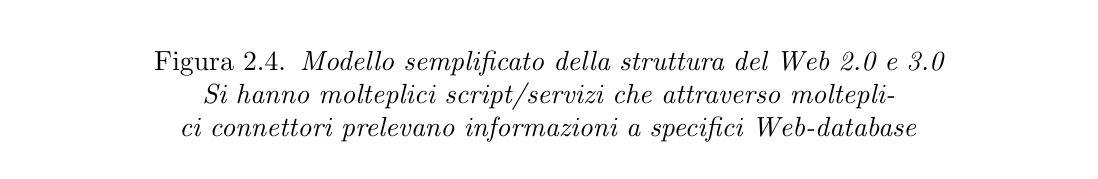
\begin{tikzpicture}
\node [align=center,text width=13cm]
        {
           \\Figura 2.4. \textit{Modello semplificato della struttura del Web 2.0 e 3.0\\ Si hanno molteplici script/servizi che attraverso molteplici connettori prelevano informazioni a specifici Web-database}
        };
\end{tikzpicture}
\end{center}
Conseguentemente al mutamento del lato server, i browser divennero  più complessi eliminando le incompatibilità che vi erano in passato con le web app ed offrendo una vasta gamma di servizi oggigiorno fondamentali. Un esempio si ha dall'arrivo di \textit{JavaScript}, per mezzo del quale si rese possibile eseguire codici direttamente sul browser. \\ Col Web 2.0 si registrò un fortissimo aumento degli utenti e dei contenuti pubblicati. Basti infatti pensare che ogni post che venisse pubblicato da qualcuno su un qualsiasi social media diventava (e diventa ancora) effettivamente un contenuto reperibile da chiunque su internet.\\\\
Passando dal Web 1.0 al 2.0 e continuando esso a crescere in modo esponenziale si è venuto a creare un problema: se prima su internet scarseggiavano i contenuti e si rischiava di non riuscire a trovare una corrispondenza alle nostre ricerche, questi divennero poi troppi e districarsi tra essi per presentare una corrispondenza significativa divenne sempre più difficile (Figura 2.5).\\\\
Il \textbf{Web 3.0}, il \textit{Web of Things}, è quello su cui oggigiorno navighiamo ed è basato sul paradigma dell'\textit{intelligenza semantica}, ancora oggi in piena evoluzione. In questa fase, il World Wide Web è rappresentato da un ambiente in cui ogni file pubblicato (pagine HTML, immagini, video, testi ecc...) entra concettualmente a far parte di un enorme database , il\textit{ Web Database} nel quale ogni dato è interpretabile tramite metadati associati ad esso che ne specificano il contesto semantico in un formato adatto all'interrogazione, all'interpretazione e, più in generale, all'elaborazione automatica intelligente. L'intelligenza è infatti la caratteristica fondamentale di questa fase. Tramite algoritmi sempre più sofisticati che sfruttano l'intelligenza artificiale avremo in futuro programmi più potenti ed efficienti capaci di interagire e collaborare tra loro e con gli utenti, sfruttando la potenza della semantica. Si pensi ad esempio se un'applicazione calendario ed una di posta elettronica fossero in grado di comunicare tra loro. Ogni volta che venisse fissato un appuntamento, il calendario potrebbe aggiornarsi da solo, tramite le informazioni comunicategli dall'applicazione di posta elettronica.\\ Per far sì che ciò sia possibile, il Web 3.0 si basa sul concetto che tutte le fonti siano codificate secondo gli stessi criteri e che quindi tutti i documenti condividano la lingua con cui sono scritti. \\
\begin{figure}[h]
\begin{center}
\includegraphics[width=14cm]{Immagini/webcontest.png}

\begin{tikzpicture}
\node [below=3cm, align=center,text width=13cm] at (stack)
        {
            Figura 2.5. \textit{Crescita della rete Internet}
        };
\end{tikzpicture} 
\end{center}
\end{figure}
La rete è in continuo mutamento e sul come si svilupperà il Web 3.0 si possono fare solo congetture.\\Tim Berners-Lee vede il Web 3.0 come una rete raggiungibile da tutti, senza barriere, che tramite la semantica possa generare applicazioni web più potenti di qualsiasi altra applicazione mai creata. Tale potenza, oltre che dal punto di vista della semantica è intesa anche dal punto di vista grafico, dove la \textit{grafica vettoriale scalabile} (SVG), secondo Lee, prenderà il sopravvento. Per mezzo di essa è possibile esprimere figure interattive che possono essere ridefinite in qualsiasi momento ed in qualsiasi punto, senza perdere un grammo di qualità. Ci sono tuttavia persone che teorizzano si tenderà a portare la rete in una forma tridimensionale (tipo second life) fatta non più di pagine ma di spazi in cui poterci muovere per trovare ciò che cerchiamo. Altre teorie vedono il futuro del web come un'entità onnipresente nella vita quotidiana, capace di alterare letteralmente le percezioni umane. Da quest'ultimo punto di vista, i Google Glass potrebbero essere visti come un primo piccolo tentativo di sviluppo, che non ha però trovato spazio nella società odierna. \\
\end{document}